\documentclass{sn-jnl}

\usepackage{graphicx}
\usepackage{amsmath}
\usepackage{amssymb}
\usepackage{booktabs}
\usepackage{multirow}
\usepackage{url}
\usepackage{hyperref}
\usepackage{tikz}
\usetikzlibrary{arrows.meta, positioning, shapes, fit}

\begin{document}

\title{From CPU-Orchestrated to GPU-Driven Storage: A Survey of GPU-Integrated I/O Architectures}

\author*[1]{\fnm{First} \sur{Author}}
\affil[1]{\orgname{Institution Name}, \orgaddress{\city{City}, \country{Country}}}

\abstract{GPU-centric computing in AI and HPC has shifted the performance bottleneck from arithmetic throughput to data orchestration across storage, memory, and interconnects. While direct-path technologies reduce copy overhead, many deployments remain constrained by CPU-centric control planes, metadata serialization, and topology-induced variability. This survey studies the architectural transition from CPU-orchestrated I/O to GPU-integrated and emerging GPU-driven storage systems. We organize the design space with a three-dimensional taxonomy based on control plane, data path, and deployment model, then map representative systems from GPU-aware filesystems to GPUDirect and disaggregated-storage deployments. Building on this taxonomy, we synthesize system design dimensions---data layout, scheduling, memory hierarchy management, and fault tolerance---and analyze how their interactions determine end-to-end behavior in training and serving pipelines. We further identify open research problems in GPU-native I/O control, storage--compute co-design, disaggregated deployment semantics, and unified APIs. The resulting framework provides a principled foundation for evaluating and designing next-generation GPU-integrated storage stacks.}

\keywords{GPU storage, I/O architecture, GPUDirect Storage, NVMe-oF, AI systems}

\maketitle

\section{Introduction}

GPU-centric computing now underpins both large-scale AI training and modern HPC simulation, and the corresponding data footprint has expanded from gigabyte-scale epochs to multi-terabyte and even petabyte-scale datasets and checkpoints. In this regime, storage and input pipelines frequently dominate end-to-end time-to-solution, even when accelerator compute is abundant. Empirical evidence from ML data-processing frameworks and distributed caching systems shows that data ingestion, shuffling, and staging can directly throttle GPU utilization if storage cannot sustain required concurrency and locality \cite{murray2021tfdata,hoard2018}. Similar pressures appear in HPC/AI production storage environments, where persistence and movement of large model states have become first-order system concerns \cite{zhang2025hpcstoragesurvey,rajbhandari2021zeroinfinity}.

The core architectural mismatch is that mainstream storage stacks were designed for CPU-centric orchestration. In traditional paths, the host CPU remains responsible for request submission, metadata handling, synchronization, and completion processing; data frequently traverses host-managed paths before reaching accelerator memory. Consequently, \emph{CPU remains on the critical path of I/O}, creating control-plane and software-path overheads that scale poorly with massively parallel GPU execution \cite{linux_io_uring,spdk_overview,nvme_spec}. For fine-grained or metadata-heavy access patterns, this mismatch manifests as low accelerator occupancy despite available storage bandwidth \cite{silberstein2013gpufs,shahar2016gpufs}.

Recent technologies have improved this situation but only partially. RDMA transports, GPUDirect RDMA, and GPUDirect Storage reduce copies and bypass host bounce buffers, yielding substantial gains in transfer efficiency \cite{infiniband_spec,nvidia_gdrdma,nvidia_gds_blog,nvidia_gds_overview}. However, most of these advances primarily optimize \emph{data movement} (where bytes flow and how fast), while leaving higher-level orchestration, metadata semantics, and control placement relatively unchanged. This is precisely why existing data-movement-centric reviews are insufficient for explaining end-to-end behavior in GPU-dominated data systems \cite{traub2023compstoragesurvey,zhang2025hpcstoragesurvey}.

This survey adopts a different perspective: the critical transition is from GPUs as passive data consumers to GPUs as active participants in storage interaction and, increasingly, storage control. We use \emph{GPU-integrated storage} to denote architectures where storage abstractions, control decisions, and data paths are co-designed around accelerator execution contexts rather than retrofitted onto CPU-first stacks. Systems such as GPUfs, BaM, and GeminiFS illustrate this shift by exposing GPU-visible storage interfaces or by pushing portions of I/O decision making closer to accelerator-driven workflows \cite{silberstein2013gpufs,qureshi2023bam,geminifs2025}.

Accordingly, the scope of this survey is \emph{not} limited to copy elimination or direct DMA paths. We cover (i) architecture-level control-plane evolution, (ii) data-path mechanisms from local to remote storage, (iii) deployment models including disaggregated and fabric-attached resources, and (iv) workload-driven requirements from AI training pipelines and checkpoint-heavy execution. This broader framing connects transport/protocol building blocks (NVMe, NVMe-oF, RDMA) with filesystem/runtime behavior and application-level bottlenecks in one system narrative \cite{nvmeof_spec,pcie_spec,liu2017rackscale,murray2021tfdata}.

Our contributions are fourfold:
\begin{enumerate}
    \item \textbf{Systematic co-evolution view.} We present a structured account of how storage and GPU subsystems have co-evolved from CPU-orchestrated paths to accelerator-participatory designs \cite{nvidia_gds_blog,silberstein2013gpufs,qureshi2023bam}.
    \item \textbf{Unified taxonomy.} We develop a taxonomy of GPU-integrated I/O architectures spanning control-plane ownership, data-path realization, deployment context, and consistency/metadata semantics.
    \item \textbf{Cross-system design synthesis.} We synthesize recurring principles and trade-offs across research prototypes, production frameworks, and standards-backed deployments \cite{geminifs2025,nvidia_gds_overview,infiniband_spec}.
    \item \textbf{GPU-driven paradigm outlook.} We analyze emerging directions in which GPUs become active storage participants, and we identify open problems for end-to-end system redesign in AI/HPC environments \cite{rajbhandari2021zeroinfinity,zhang2025hpcstoragesurvey}.
\end{enumerate}

\section{Related Work}

\subsection{Surveys and position papers}

Existing surveys and position papers provide important context but typically emphasize either broad HPC storage evolution or computational storage offload, rather than GPU-centered storage-stack evolution as a unified architectural problem. For example, recent HPC storage surveys summarize filesystems, deployment models, and protocol trends, while computational-storage surveys focus on where computation should execute in the storage hierarchy; neither thread fully models GPU-driven control-path transitions across local and remote I/O domains \cite{zhang2025hpcstoragesurvey,traub2023compstoragesurvey,liu2017rackscale}. As a result, prior surveys are valuable baselines but leave a synthesis gap at the intersection of accelerator control, storage semantics, and workload-coupled data services \cite{murray2021tfdata,rajbhandari2021zeroinfinity}.

\subsection{Traditional CPU-orchestrated storage systems}

Traditional POSIX-oriented stacks and host-managed I/O software place the CPU on the critical path for request submission, metadata handling, and completion processing, which becomes increasingly expensive as accelerator throughput grows. Even when optimized user-space paths are used, control-plane work remains primarily host-centric, so GPUs still observe indirect storage service and coordination overheads \cite{linux_io_uring,spdk_overview,nvme_spec}. This CPU-first orchestration model is one root cause of low accelerator utilization under data-intensive pipelines, especially when many small operations amplify control and synchronization costs \cite{murray2021tfdata,hoard2018}.

\subsection{GPU-aware and GPU-integrated storage systems}

GPU-aware file and runtime systems moved beyond host-only orchestration by exposing storage abstractions to GPU execution contexts and by co-designing data access with accelerator behavior. GPUfs and follow-up work demonstrated that GPU-side file access is feasible but requires careful handling of consistency, granularity, and control interactions; newer systems such as GeminiFS further align filesystem behavior with GPU-dominated workflows \cite{silberstein2013gpufs,shahar2016gpufs,geminifs2025}. These efforts are architecturally significant because they begin to redefine storage as a subsystem co-evolving with accelerator scheduling, not merely a backend byte source \cite{qureshi2023bam,qiu2025geminifs}.

\subsection{GPU direct and bypass I/O mechanisms}

Bypass mechanisms (GPUDirect RDMA and GPUDirect Storage) substantially reduce host bounce buffering and improve transfer efficiency, and they are now foundational in production heterogeneous clusters. However, this line of work is primarily data-path-centric: it optimizes copy avoidance and transport efficiency but often assumes largely unchanged control and metadata planes above the transport layer \cite{nvidia_gdrdma,nvidia_gds_blog,nvidia_gds_overview,nvidia_gds_best_practices}. Consequently, bypass I/O is necessary but insufficient for explaining end-to-end architectural evolution from CPU-mediated orchestration to GPU-participatory storage control \cite{pcie_spec,infiniband_spec,nvmeof_spec}.

\subsection{Storage for AI workloads}

AI input pipelines, distributed caching, and model-state persistence reveal workload properties that differ sharply from assumptions in conventional enterprise and HPC storage tuning. tf.data and Hoard show that data loading, prefetching, and locality decisions can dominate training throughput, while memory-tiering/checkpoint work shows that persistence policies directly affect model scale and recovery behavior \cite{murray2021tfdata,hoard2018,rajbhandari2021zeroinfinity}. These results suggest that storage architecture for GPU clusters must be co-designed with pipeline structure and training dynamics, rather than optimized as an isolated block-I/O subsystem \cite{hdf5gds2020,geminifs2025}.

\subsection{Disaggregated and remote storage for accelerators}

Disaggregated storage and remote-access protocols provide elasticity and pooling that are increasingly relevant for accelerator clusters, where local capacity is insufficient for multi-tenant AI and HPC workloads. NVMe-oF/RDMA fabrics and rack-scale disaggregation studies establish the deployment substrate for remote SSD access, but GPU-visible semantics and control-path placement remain underdeveloped compared with transport maturity \cite{nvmeof_spec,infiniband_spec,liu2017rackscale}. Thus, remote storage research contributes critical building blocks while still leaving open questions about GPU-initiated scheduling, metadata locality, and end-to-end coordination \cite{qureshi2023bam,nvidia_gdrdma}.

\subsection{Summary and gap identification}

Across these lines of work, the dominant emphasis is on optimizing \emph{how data moves} (copy elimination, DMA efficiency, transport throughput), while comparatively fewer studies address \emph{how storage control evolves} when GPUs become active participants in I/O orchestration. In particular, control-plane evolution, GPU-resident storage participation, and full end-to-end co-design across data, metadata, and workload pipelines remain fragmented across separate communities and artifacts \cite{nvidia_gds_overview,silberstein2013gpufs,qureshi2023bam,murray2021tfdata}. Therefore, a unified survey is needed to connect CPU-orchestrated stacks, GPU-aware integration, direct/bypass paths, and emerging GPU-driven storage paradigms within one architectural framework \cite{geminifs2025,zhang2025hpcstoragesurvey,traub2023compstoragesurvey}.

\section{A Taxonomy of GPU-Integrated I/O Architectures}

We classify designs along four orthogonal axes.

\subsection{Axis I: Control-plane ownership}

\textbf{CPU-orchestrated designs} retain host control over submission, completion handling, and queue scheduling. \textbf{Hybrid designs} preserve host policy but expose direct GPU-resident data paths. \textbf{GPU-driven designs} push portions of request generation and scheduling onto device-side execution contexts \cite{silberstein2013gpufs,bam2024}.

\subsection{Axis II: Data-plane placement}

Data transfer can be staged through host DRAM or placed on direct DMA paths to GPU memory. Direct placement reduces redundant copies but can expose fine-grain access inefficiencies when request sizes are too small or alignment is poor \cite{nvidia_gds_best_practices}.

\subsection{Axis III: Transport realization}

Transport options include local PCIe-attached NVMe, RDMA-backed remote block paths, and composable disaggregated fabrics. The transport choice interacts with queue depth, completion latency variance, and backpressure behavior \cite{nvme_spec,infiniband_spec,cxl_spec}.

\subsection{Axis IV: Consistency and metadata semantics}

Architectures diverge in metadata handling: host-side POSIX mediation, user-space poll-mode stacks, and GPU-visible metadata caches. The critical path often depends more on metadata round-trips than on raw bandwidth, especially for small object workloads \cite{spdk_overview,geminifs2025}.

\begin{figure}[t]
  \centering
  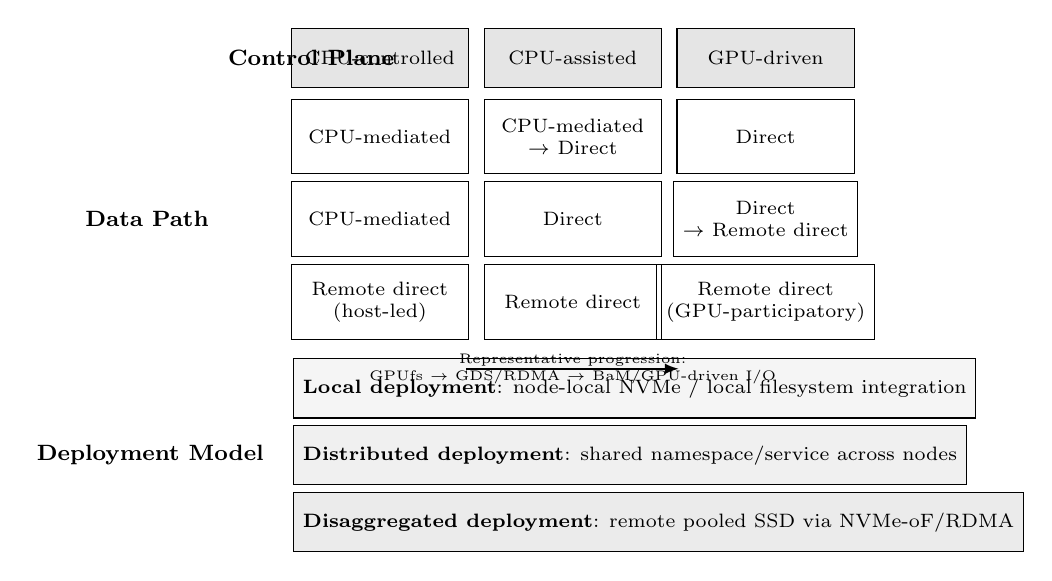
\begin{tikzpicture}[
  font=\scriptsize,
  cell/.style={draw, minimum width=2.25cm, minimum height=0.95cm, align=center},
  hdr/.style={draw, fill=gray!20, minimum width=2.25cm, minimum height=0.75cm, align=center},
  band/.style={draw, minimum width=7.15cm, minimum height=0.75cm, align=left},
  arr/.style={-{Latex[length=1.8mm]}, thick}
]

% headers
\node[hdr] (h1) at (0,0) {CPU-controlled};
\node[hdr] (h2) at (2.45,0) {CPU-assisted};
\node[hdr] (h3) at (4.90,0) {GPU-driven};
\node[anchor=west,font=\footnotesize] at (-2.05,0) {\textbf{Control Plane}};

% rows
\node[cell] (r11) at (0,-1.0) {CPU-mediated};
\node[cell] (r12) at (2.45,-1.0) {CPU-mediated\\$\rightarrow$ Direct};
\node[cell] (r13) at (4.90,-1.0) {Direct};

\node[cell] (r21) at (0,-2.05) {CPU-mediated};
\node[cell] (r22) at (2.45,-2.05) {Direct};
\node[cell] (r23) at (4.90,-2.05) {Direct\\$\rightarrow$ Remote direct};

\node[cell] (r31) at (0,-3.10) {Remote direct\\(host-led)};
\node[cell] (r32) at (2.45,-3.10) {Remote direct};
\node[cell] (r33) at (4.90,-3.10) {Remote direct\\(GPU-participatory)};

\node[anchor=east, font=\footnotesize, align=right] at (-2.05,-2.05) {\textbf{Data Path}};

% deployment bands
\node[band, fill=gray!8, anchor=west] (b1) at (-1.10,-4.20) {\textbf{Local deployment}: node-local NVMe / local filesystem integration};
\node[band, fill=gray!12, anchor=west] (b2) at (-1.10,-5.05) {\textbf{Distributed deployment}: shared namespace/service across nodes};
\node[band, fill=gray!16, anchor=west] (b3) at (-1.10,-5.90) {\textbf{Disaggregated deployment}: remote pooled SSD via NVMe-oF/RDMA};
\node[anchor=east,font=\footnotesize] at (-1.35,-5.05) {\textbf{Deployment Model}};

% mapping hints
\node[font=\tiny, align=center] at (2.45,-3.95) {Representative progression:\\GPUfs $\rightarrow$ GDS/RDMA $\rightarrow$ BaM/GPU-driven I/O};
\draw[arr] (1.1,-3.95) -- (3.8,-3.95);

\end{tikzpicture}

  \caption{Survey taxonomy from CPU-orchestrated to GPU-driven storage architectures.}
  \label{fig:taxonomy}
\end{figure}

\section{Figures}

\begin{figure*}[t]
\centering
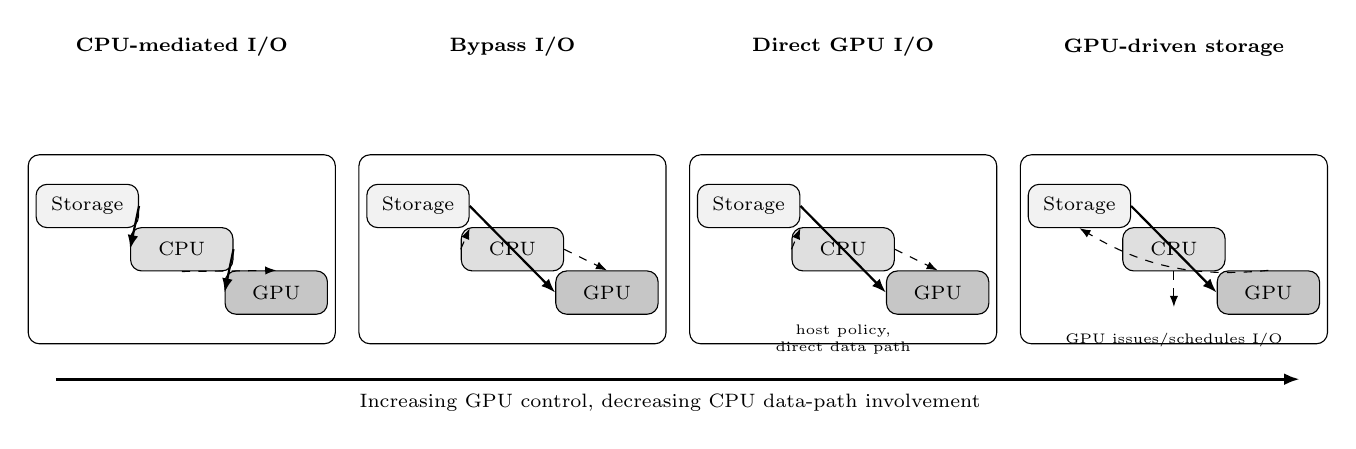
\begin{tikzpicture}[
  x=1cm,y=1cm,
  box/.style={draw, rounded corners, minimum width=1.3cm, minimum height=0.55cm, align=center, font=\scriptsize},
  stage/.style={draw, rounded corners, minimum width=3.9cm, minimum height=2.4cm},
  data/.style={-{Latex[length=1.8mm]}, thick},
  ctrl/.style={-{Latex[length=1.4mm]}, dashed, thin}
]

% stage frames
\node[stage] (s1) at (0,0) {};
\node[stage] (s2) at (4.2,0) {};
\node[stage] (s3) at (8.4,0) {};
\node[stage] (s4) at (12.6,0) {};

\node[font=\scriptsize, above=1.12cm] at (s1.north) {\textbf{CPU-mediated I/O}};
\node[font=\scriptsize, above=1.12cm] at (s2.north) {\textbf{Bypass I/O}};
\node[font=\scriptsize, above=1.12cm] at (s3.north) {\textbf{Direct GPU I/O}};
\node[font=\scriptsize, above=1.12cm] at (s4.north) {\textbf{GPU-driven storage}};

% components
\node[box, fill=gray!10] (st1) at (-1.2,0.55) {Storage};
\node[box, fill=gray!25] (cpu1) at (0,0.0) {CPU};
\node[box, fill=gray!45] (gpu1) at (1.2,-0.55) {GPU};

\node[box, fill=gray!10] (st2) at (3.0,0.55) {Storage};
\node[box, fill=gray!25] (cpu2) at (4.2,0.0) {CPU};
\node[box, fill=gray!45] (gpu2) at (5.4,-0.55) {GPU};

\node[box, fill=gray!10] (st3) at (7.2,0.55) {Storage};
\node[box, fill=gray!25] (cpu3) at (8.4,0.0) {CPU};
\node[box, fill=gray!45] (gpu3) at (9.6,-0.55) {GPU};

\node[box, fill=gray!10] (st4) at (11.4,0.55) {Storage};
\node[box, fill=gray!25] (cpu4) at (12.6,0.0) {CPU};
\node[box, fill=gray!45] (gpu4) at (13.8,-0.55) {GPU};

% stage 1
\draw[data] (st1.east) -- (cpu1.west);
\draw[data] (cpu1.east) -- (gpu1.west);
\draw[ctrl] (cpu1.south) -- (gpu1.north);

% stage 2
\draw[data] (st2.east) -- (gpu2.west);
\draw[ctrl] (cpu2.west) -- (st2.south east);
\draw[ctrl] (cpu2.east) -- (gpu2.north);

% stage 3
\draw[data] (st3.east) -- (gpu3.west);
\draw[ctrl] (cpu3.east) -- (gpu3.north);
\draw[ctrl] (cpu3.west) -- (st3.south east);
\node[font=\tiny, align=center] at (8.4,-1.15) {host policy,\\ direct data path};

% stage 4
\draw[data] (st4.east) -- (gpu4.west);
\draw[ctrl] (gpu4.north) to[bend left=18] (st4.south);
\draw[ctrl] (cpu4.south) -- ++(0,-0.45);
\node[font=\tiny] at (12.6,-1.15) {GPU issues/schedules I/O};

\draw[-{Latex[length=2mm]}, very thick] (-1.6,-1.65) -- (14.2,-1.65);
\node[font=\scriptsize] at (6.2,-1.95) {Increasing GPU control, decreasing CPU data-path involvement};

\end{tikzpicture}

\caption{Evolution of storage--GPU interaction from CPU-mediated I/O to GPU-driven storage. The progression highlights two concurrent trends: (i) gradual removal of CPU from the data path, and (ii) increasing GPU participation in I/O control.}
\label{fig:evolution}
\end{figure*}

\begin{figure*}[t]
\centering
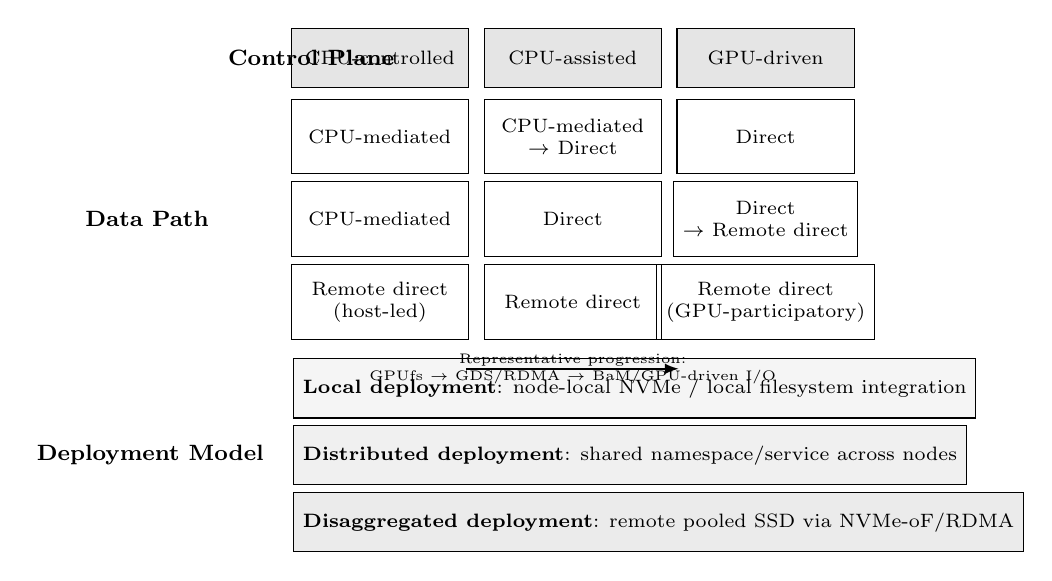
\begin{tikzpicture}[
  font=\scriptsize,
  cell/.style={draw, minimum width=2.25cm, minimum height=0.95cm, align=center},
  hdr/.style={draw, fill=gray!20, minimum width=2.25cm, minimum height=0.75cm, align=center},
  band/.style={draw, minimum width=7.15cm, minimum height=0.75cm, align=left},
  arr/.style={-{Latex[length=1.8mm]}, thick}
]

% headers
\node[hdr] (h1) at (0,0) {CPU-controlled};
\node[hdr] (h2) at (2.45,0) {CPU-assisted};
\node[hdr] (h3) at (4.90,0) {GPU-driven};
\node[anchor=west,font=\footnotesize] at (-2.05,0) {\textbf{Control Plane}};

% rows
\node[cell] (r11) at (0,-1.0) {CPU-mediated};
\node[cell] (r12) at (2.45,-1.0) {CPU-mediated\\$\rightarrow$ Direct};
\node[cell] (r13) at (4.90,-1.0) {Direct};

\node[cell] (r21) at (0,-2.05) {CPU-mediated};
\node[cell] (r22) at (2.45,-2.05) {Direct};
\node[cell] (r23) at (4.90,-2.05) {Direct\\$\rightarrow$ Remote direct};

\node[cell] (r31) at (0,-3.10) {Remote direct\\(host-led)};
\node[cell] (r32) at (2.45,-3.10) {Remote direct};
\node[cell] (r33) at (4.90,-3.10) {Remote direct\\(GPU-participatory)};

\node[anchor=east, font=\footnotesize, align=right] at (-2.05,-2.05) {\textbf{Data Path}};

% deployment bands
\node[band, fill=gray!8, anchor=west] (b1) at (-1.10,-4.20) {\textbf{Local deployment}: node-local NVMe / local filesystem integration};
\node[band, fill=gray!12, anchor=west] (b2) at (-1.10,-5.05) {\textbf{Distributed deployment}: shared namespace/service across nodes};
\node[band, fill=gray!16, anchor=west] (b3) at (-1.10,-5.90) {\textbf{Disaggregated deployment}: remote pooled SSD via NVMe-oF/RDMA};
\node[anchor=east,font=\footnotesize] at (-1.35,-5.05) {\textbf{Deployment Model}};

% mapping hints
\node[font=\tiny, align=center] at (2.45,-3.95) {Representative progression:\\GPUfs $\rightarrow$ GDS/RDMA $\rightarrow$ BaM/GPU-driven I/O};
\draw[arr] (1.1,-3.95) -- (3.8,-3.95);

\end{tikzpicture}

\caption{Core taxonomy of GPU-integrated I/O architectures across three dimensions: control plane, data path, and deployment model. The layout is structured to map architectural states without introducing categories beyond the taxonomy definitions used in this survey.}
\label{fig:taxonomy}
\end{figure*}

\begin{figure*}[t]
\centering
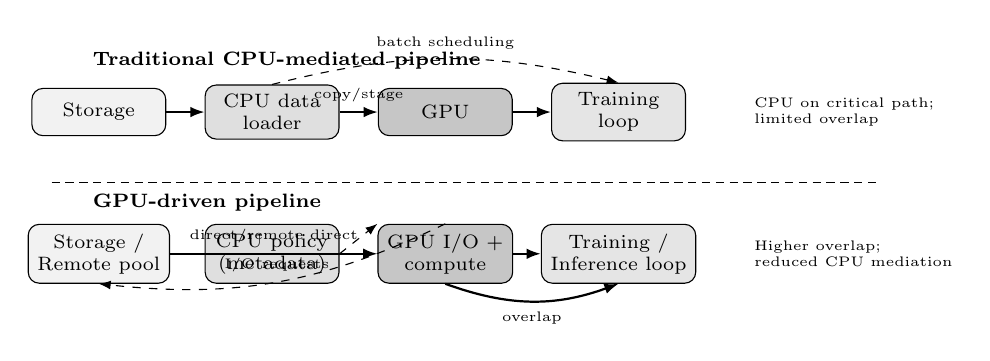
\begin{tikzpicture}[
  x=1cm,y=1cm,
  box/.style={draw, rounded corners, minimum width=1.7cm, minimum height=0.6cm, align=center, font=\scriptsize},
  data/.style={-{Latex[length=1.8mm]}, thick},
  ctrl/.style={-{Latex[length=1.5mm]}, dashed, thin}
]

% top: traditional
\node[font=\scriptsize, anchor=west] at (-0.2,1.65) {\textbf{Traditional CPU-mediated pipeline}};
\node[box, fill=gray!10] (tstor) at (0,1.0) {Storage};
\node[box, fill=gray!25] (tcpu) at (2.2,1.0) {CPU data\\loader};
\node[box, fill=gray!45] (tgpu) at (4.4,1.0) {GPU};
\node[box, fill=gray!20] (tloop) at (6.6,1.0) {Training\\loop};
\draw[data] (tstor.east) -- (tcpu.west);
\draw[data] (tcpu.east) -- node[above,font=\tiny]{copy/stage} (tgpu.west);
\draw[data] (tgpu.east) -- (tloop.west);
\draw[ctrl] (tcpu.north) to[bend left=14] node[above,font=\tiny]{batch scheduling} (tloop.north);
\node[font=\tiny, align=left, anchor=west] at (8.2,1.0) {CPU on critical path;\\ limited overlap};

% bottom: gpu-driven
\node[font=\scriptsize, anchor=west] at (-0.2,-0.15) {\textbf{GPU-driven pipeline}};
\node[box, fill=gray!10] (gstor) at (0,-0.8) {Storage /\\Remote pool};
\node[box, fill=gray!25] (gcpu) at (2.2,-0.8) {CPU policy\\(metadata)};
\node[box, fill=gray!45] (ggpu) at (4.4,-0.8) {GPU I/O +\\compute};
\node[box, fill=gray!20] (gloop) at (6.6,-0.8) {Training /\\Inference loop};
\draw[data] (gstor.east) -- node[above,font=\tiny]{direct/remote direct} (ggpu.west);
\draw[data] (ggpu.east) -- (gloop.west);
\draw[ctrl] (gcpu.east) -- (ggpu.north west);
\draw[ctrl] (ggpu.north) to[bend left=16] node[above,font=\tiny]{I/O requests} (gstor.south);
\draw[data] (ggpu.south) to[bend right=20] node[below,font=\tiny]{overlap} (gloop.south);
\node[font=\tiny, align=left, anchor=west] at (8.2,-0.8) {Higher overlap;\\ reduced CPU mediation};

% separator
\draw[densely dashed] (-0.6,0.1) -- (9.9,0.1);

\end{tikzpicture}

\caption{Comparison of traditional CPU-mediated and GPU-driven AI pipelines. The lower path illustrates direct/remote-direct data movement and tighter compute--I/O overlap, while the CPU remains focused on policy and metadata coordination.}
\label{fig:pipeline}
\end{figure*}

\section{System Design Dimensions}\label{sec:design-anchor}

This section translates the taxonomy in Section~\ref{sec:taxonomy-anchor} into an actionable design space. We focus on four dimensions that repeatedly determine end-to-end performance in GPU-integrated storage systems: data layout, I/O scheduling, memory management, and fault tolerance. In each dimension, the right choice depends on the same architectural tuple $\{\text{control plane, data path, deployment}\}$ used in our taxonomy \cite{silberstein2013gpufs,nvidia_gds_overview,qureshi2023bam,geminifs2025}.

\subsection{Data Layout}

\textbf{Design problem.} Data layout determines whether GPU-side access is predominantly sequential, strided, or random, and therefore whether a system can exploit direct-path bandwidth or remains bounded by small-request control overheads. In practice, layout decisions span sample sharding, tensor serialization, and checkpoint object granularity, and they interact strongly with deployment (local versus distributed/disaggregated storage) \cite{murray2021tfdata,hoard2018,zhang2025hpcstoragesurvey}.

\textbf{Alternative approaches.} Sequential shard-oriented layouts reduce seek and metadata pressure, favoring CPU-mediated and direct paths in throughput-oriented training phases. Fine-grained sample-level or object-level layouts improve flexibility for skewed sampling and elastic serving, but they amplify metadata and scheduling costs, especially in remote direct paths over NVMe-oF/RDMA \cite{nvmeof_spec,infiniband_spec,liu2017rackscale}. Checkpoint layouts follow a similar pattern: monolithic snapshots simplify recovery semantics, while partitioned/incremental representations improve write parallelism and overlap opportunities with GPU compute \cite{rajbhandari2021zeroinfinity,geminifs2025}.

\textbf{Trade-offs.} Layout design is a three-way trade-off among (i) sequential efficiency, (ii) runtime flexibility, and (iii) preprocessing burden. Preprocessing-heavy layouts can substantially improve steady-state GPU feed rate, but reduce agility under dynamic workloads. Conversely, highly flexible layouts increase random access and control-plane amplification, which is particularly costly when control remains CPU-dominant \cite{murray2021tfdata,qureshi2023bam}.

\subsection{I/O Scheduling}

\textbf{Design problem.} I/O scheduling decides when and where requests are issued, how queue depth is controlled, and how transfers are overlapped with compute. This is fundamentally a control-plane question: host-driven schedulers are mature and predictable, while GPU-aware scheduling can reduce reaction latency for fine-grained pipelines but requires tighter runtime integration \cite{linux_io_uring,spdk_overview,silberstein2013gpufs}.

\textbf{Alternative approaches.} CPU-driven prefetch pipelines (e.g., host data-loader centric) remain common because they preserve software compatibility and centralized policy control. Hybrid approaches couple host policy with direct paths (GDS/RDMA), using asynchronous submission to increase overlap while retaining host metadata authority \cite{nvidia_gds_blog,nvidia_gds_overview,nvidia_gdrdma}. Emerging GPU-participatory designs push request generation and demand signaling closer to kernels, reducing control lag but increasing complexity in fairness and coordination \cite{qureshi2023bam,geminifs2025}.

\textbf{Trade-offs.} Throughput-oriented scheduling favors deep queues and aggressive prefetching; latency-sensitive phases favor tighter pacing and smaller in-flight windows. The practical frontier is scheduling complexity versus benefit: richer dependency-aware schedules can improve overlap but also increase synchronization overhead across CPU/GPU domains. Where data paths are remote-direct, queue misconfiguration can quickly convert bandwidth headroom into tail-latency instability \cite{nvmeof_spec,infiniband_spec,liu2017rackscale}.

\subsection{Memory Management}

\textbf{Design problem.} Memory policy determines whether I/O improvements translate into application speedups. Pinned host buffers, registration caches, GPU-resident caching, and multi-tier placement (GPU/CPU/SSD) jointly define copy count, hit rate, and eviction behavior. This dimension couples directly to data-path realization and to control responsibility for placement decisions \cite{nvidia_gds_best_practices,nvidia_gdrdma,rajbhandari2021zeroinfinity}.

\textbf{Alternative approaches.} CPU-mediated stacks often rely on host staging buffers and explicit host-to-device copies; direct-path systems reduce staging but still need careful pinning/registration management. GPU-side caches (including serving-time KV caches) reduce repeated storage accesses but shift pressure to device memory management and eviction policy \cite{nvidia_gds_overview,kwon2023vllm,zhong2024distserve}. Hierarchical memory/offload schemes extend effective capacity by moving states across GPU, CPU, and SSD tiers, improving scale at the cost of added placement and consistency complexity \cite{rajbhandari2021zeroinfinity,geminifs2025}.

\textbf{Trade-offs.} Larger caches and pinned regions improve throughput and overlap but reduce usable memory for compute and can increase fragmentation. Aggressive offload lowers device pressure but can introduce bursty transfers and control jitter. The central trade-off is memory efficiency versus performance predictability under mixed training/serving workloads \cite{kwon2023vllm,nvidia_gds_best_practices,murray2021tfdata}.

\subsection{Fault Tolerance}

\textbf{Design problem.} Fault tolerance must preserve correctness without collapsing the compute--I/O overlap benefits of GPU-centric pipelines. Checkpointing frequency, checkpoint granularity, and recovery protocol all feed back into control-plane load, data-path occupancy, and deployment-level storage contention \cite{rajbhandari2021zeroinfinity,zhang2025hpcstoragesurvey}.

\textbf{Alternative approaches.} Full synchronous checkpoints simplify consistency and recovery logic but create large pause windows and peak bandwidth bursts. Incremental or asynchronous persistence reduces stall time and can overlap with GPU compute, but requires metadata tracking and stronger ordering discipline across tiers and nodes \cite{hdf5gds2020,geminifs2025}. In disaggregated deployments, recovery design additionally depends on fabric behavior and tenant isolation policy, not only on local write throughput \cite{nvmeof_spec,liu2017rackscale,infiniband_spec}.

\textbf{Trade-offs.} Lower recovery-point objectives usually imply higher checkpoint traffic and storage cost. Relaxing synchronization improves runtime performance but complicates replay semantics and increases recovery-time uncertainty. Systems therefore face explicit consistency-versus-performance decisions that should be aligned with control authority placement and deployment model \cite{rajbhandari2021zeroinfinity,hdf5gds2020,geminifs2025}.

\paragraph{Cross-cutting synthesis.}
These four dimensions are tightly coupled: layout choices shape scheduling granularity; scheduling policy determines memory pressure; memory policy constrains feasible checkpoint strategies; and fault-tolerance mechanisms feed back into both control and data-path occupancy. Across systems, the same bottlenecks recur---CPU orchestration overhead, data-movement amplification, and limited GPU-native I/O control---indicating that local optimizations are insufficient without end-to-end co-design across control plane, data path, and deployment model \cite{qureshi2023bam,nvidia_gds_overview,murray2021tfdata,geminifs2025}.

\section{AI Workloads and Storage Implications}

Modern AI pipelines expose storage behaviors that differ from traditional throughput benchmarks: training emphasizes sustained ingest and periodic persistence, whereas serving emphasizes low-latency state access with bursty phase shifts. In both regimes, GPU utilization depends on whether storage and runtime policies are co-designed around compute phases rather than treated as independent subsystems \cite{murray2021tfdata,hoard2018,kwon2023vllm,zhong2024distserve}.

For training, data loading, shuffling, and checkpoint traffic compete for bandwidth and control resources. Systems that optimize only one stage (e.g., ingest throughput) frequently degrade another stage (e.g., checkpoint latency), leading to unstable step time and reduced cluster efficiency \cite{rajbhandari2021zeroinfinity,geminifs2025}. This motivates architecture-level coordination across layout, scheduling, and persistence dimensions introduced in Sections~\ref{sec:taxonomy-anchor} and \ref{sec:design-anchor}.

For inference, long-context and high-concurrency serving amplify memory--storage hierarchy pressure, especially when KV/state footprints exceed device-local capacity. Remote/direct paths can relieve local pressure, but only if control and placement decisions are topology-aware and phase-aware \cite{nvidia_gdrdma,nvmeof_spec,liu2017rackscale}. Figure~\ref{fig:pipeline} summarizes the shift from CPU-mediated pipelines toward GPU-driven overlap-centric execution.

\section{Future Directions}

\subsection{GPU-driven I/O control as a first-class systems problem}

\textbf{Problem statement.} Most deployed stacks remain CPU-controlled or CPU-assisted even when data paths are direct, so GPUs still cannot reliably initiate, prioritize, and complete storage operations under a unified runtime policy. This gap arises because current interfaces separate accelerator kernels from storage queue control and metadata coordination \cite{nvidia_gds_overview,nvidia_gdrdma,linux_io_uring}.

\textbf{Why it matters.} As workloads move toward finer-grained and phase-coupled pipelines, control latency increasingly dominates transfer latency; host-side orchestration then becomes the primary bottleneck despite high raw bandwidth \cite{murray2021tfdata,qureshi2023bam}. \textbf{Taxonomy linkage:} control plane + data path.

\textbf{Limitations of existing approaches.} GPUDirect mechanisms reduce copies but do not by themselves provide GPU-native scheduling and fairness control across competing flows \cite{nvidia_gds_blog,nvidia_gds_best_practices}. \textbf{Research opportunities.} Design GPU-visible submission/completion abstractions with explicit protection domains, priority classes, and preemption semantics that remain interoperable with host safety policies.

\subsection{End-to-end storage--compute co-design for training and serving}

\textbf{Problem statement.} Current systems optimize storage and compute subsystems in isolation, while modern AI pipelines require joint optimization of sharding, prefetch depth, batch formation, and kernel scheduling. The mismatch is structural: storage interfaces expose block/object primitives, whereas training/inference runtimes reason in tensor and step semantics \cite{murray2021tfdata,hoard2018,kwon2023vllm}.

\textbf{Why it matters.} Without co-design, systems over-provision one layer (e.g., storage throughput) while under-utilizing end-to-end pipeline overlap, producing unstable throughput and poor cost efficiency \cite{zhong2024distserve,rajbhandari2021zeroinfinity}. \textbf{Taxonomy linkage:} control plane + deployment model.

\textbf{Limitations of existing approaches.} Existing frameworks expose partial pipeline controls but lack cross-layer contracts tying storage readiness to GPU execution windows \cite{murray2021tfdata,geminifs2025}. \textbf{Research opportunities.} Develop step-aware I/O intent APIs, runtime feedback loops, and schedulers that jointly optimize compute launch, data staging, and persistence at cluster scale.

\subsection{Disaggregated storage for GPU workloads beyond transport optimization}

\textbf{Problem statement.} NVMe-oF/RDMA enables storage pooling, but disaggregated deployments introduce tail latency, congestion coupling, and isolation challenges not captured by local-direct path models \cite{nvmeof_spec,infiniband_spec,liu2017rackscale}.

\textbf{Why it matters.} GPU clusters increasingly rely on pooled storage for elasticity and multi-tenancy; uncontrolled variance directly reduces accelerator utilization and service-level predictability \cite{zhang2025hpcstoragesurvey,zhong2024distserve}. \textbf{Taxonomy linkage:} deployment model + data path.

\textbf{Limitations of existing approaches.} Most current work emphasizes fabric throughput and protocol correctness, with limited support for GPU-aware admission control, placement, and noisy-neighbor isolation \cite{nvmeof_spec,liu2017rackscale}. \textbf{Research opportunities.} Build placement/scheduling policies that are topology-aware, tenant-aware, and GPU-phase-aware, plus recovery-aware routing for remote direct paths.

\subsection{Data movement minimization as a layout and runtime co-optimization problem}

\textbf{Problem statement.} Copy amplification persists across CPU memory, pinned staging regions, and GPU memory because layout decisions and runtime scheduling are often made independently. Direct path availability does not guarantee minimal movement when formats and access granularity are mismatched \cite{nvidia_gds_overview,nvidia_gds_best_practices,silberstein2013gpufs}.

\textbf{Why it matters.} Extra copies consume bandwidth, increase synchronization overhead, and reduce overlap opportunities in both training and serving paths \cite{murray2021tfdata,kwon2023vllm}. \textbf{Taxonomy linkage:} data path + control plane.

\textbf{Limitations of existing approaches.} Existing optimizations are often static (offline layout tuning) or local (single-stage copy elimination) and fail under dynamic data skew and workload phase shifts \cite{hoard2018,geminifs2025}. \textbf{Research opportunities.} Co-design adaptive layout transforms, online prefetch granularity control, and access-pattern-guided placement that explicitly optimize end-to-end copy count.

\subsection{Memory--storage hierarchy design for LLM-era systems}

\textbf{Problem statement.} LLM workloads stress hierarchical capacity and bandwidth across GPU memory, host memory, and SSD tiers, especially under large KV caches and long-context serving. Current policies often treat these tiers as loosely coupled fallbacks rather than coordinated resources \cite{kwon2023vllm,zhong2024distserve,rajbhandari2021zeroinfinity}.

\textbf{Why it matters.} Poor tier coordination leads to bursty eviction/offload traffic, unstable latency, and underutilized accelerators in both training checkpoints and inference-time state management \cite{rajbhandari2021zeroinfinity,nvidia_gdrdma}. \textbf{Taxonomy linkage:} data path + deployment model.

\textbf{Limitations of existing approaches.} Existing memory managers optimize either serving-time cache locality or training-time offload, but seldom provide a unified policy with explicit storage-awareness and recovery-awareness \cite{kwon2023vllm,geminifs2025}. \textbf{Research opportunities.} Design unified tier managers that expose predictable QoS envelopes, support state-aware migration, and couple cache policy with persistent layout decisions.

\subsection{Fault tolerance for GPU pipelines with low interruption budgets}

\textbf{Problem statement.} Checkpoint and recovery mechanisms remain expensive because persistence semantics are not co-designed with GPU execution phases and storage topology. Full synchronous checkpoints are simple but create large stall windows; asynchronous alternatives complicate ordering and replay \cite{hdf5gds2020,rajbhandari2021zeroinfinity}.

\textbf{Why it matters.} At cluster scale, checkpoint overhead and recovery delay directly translate into lost accelerator-hours and reduced service availability \cite{zhang2025hpcstoragesurvey,geminifs2025}. \textbf{Taxonomy linkage:} control plane + deployment model.

\textbf{Limitations of existing approaches.} Most systems provide either fast writes without strong replay contracts or strong semantics with high pause cost \cite{hdf5gds2020,rajbhandari2021zeroinfinity}. \textbf{Research opportunities.} Develop phase-aware incremental persistence, topology-aware redundancy placement, and verification-friendly replay protocols for GPU-driven execution graphs.

\subsection{Programming model and API gap for GPU-integrated storage}

\textbf{Problem statement.} There is no widely adopted programming model that unifies data placement intent, I/O scheduling intent, and consistency intent across CPU-mediated, direct, and remote-direct modes. Developers therefore compose ad hoc APIs, which reduces portability and obscures optimization opportunities \cite{silberstein2013gpufs,nvidia_gds_overview,spdk_overview}.

\textbf{Why it matters.} Without stable abstractions, system advances are difficult to transfer across frameworks, filesystems, and fabrics, slowing ecosystem-level progress \cite{traub2023compstoragesurvey,zhang2025hpcstoragesurvey}. \textbf{Taxonomy linkage:} all three dimensions.

\textbf{Limitations of existing approaches.} Current interfaces are fragmented by layer (runtime, filesystem, transport), with inconsistent semantics for ordering, completion, and failure handling \cite{nvidia_gdrdma,nvmeof_spec}. \textbf{Research opportunities.} Define an intent-based API stack with explicit contracts for control authority, copy semantics, and recovery behavior, plus portable conformance tests.

\paragraph{Cross-cutting synthesis.}
Across these problems, common root causes are clear: CPU-centric control persists even when data paths modernize; data movement is optimized locally rather than end-to-end; and GPU-native abstractions remain immature. Future progress therefore depends on co-designing control, data path, and deployment policies as one system, rather than treating transport acceleration as a complete solution \cite{qureshi2023bam,nvidia_gds_overview,geminifs2025,murray2021tfdata}.

\section{Conclusion}

GPU-integrated I/O is transitioning from CPU-orchestrated staging toward GPU-driven control and direct data movement. The central lesson from recent systems is not that host CPUs become irrelevant, but that host responsibilities must be narrowed to policy, protection, and coordination while performance-critical data paths are restructured around accelerator locality. The taxonomy and insights in this survey aim to support principled design choices for next-generation storage stacks that are both high-throughput and operationally robust.


\bibliography{references}

\end{document}
